\chapter{农民生活水平}
\label{chapter:famer}
农民作为农村的主体,不仅是农业生产的直接参与者,也是乡村社会结构的基础。因此,农民的生活水平是衡量农村经济和社会发展的重要指标,农民生活条件的改善直接影响到农村的可持续发展。
\section{农村就业}
\subsection{就业结构改善}
随着经济全球化的深入发展和内需市场的不断扩大,科学技术取得显著进步,农民对于提高生活质量的追求日益增强。同时,农民对新知识和新技术的接受度也显著提高,城乡之间的互动更加频繁和深入。这些因素共同作用,推动了农村产业结构的多元化发展。

\begin{figure}[h]
    \centering
    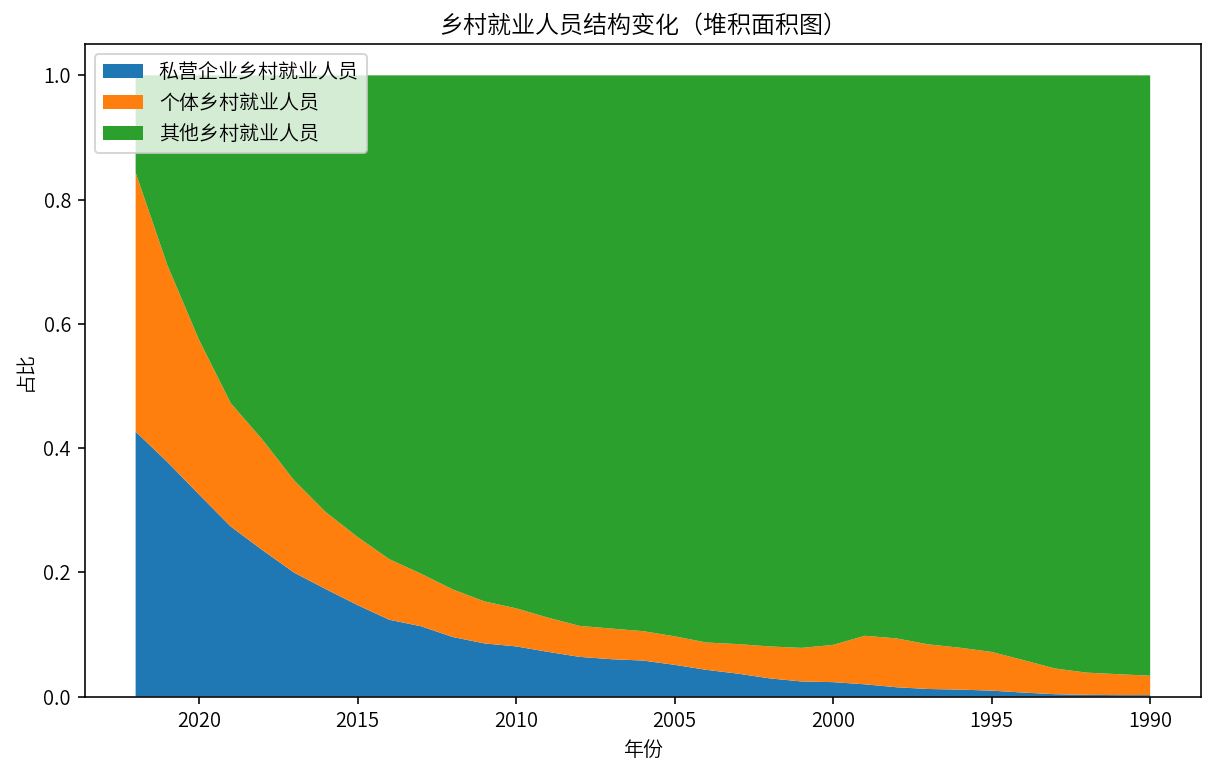
\includegraphics[width=0.75\linewidth]{figures/20.png}
    \caption{农村产业结构变化}
    \label{fig:struct_change}
\end{figure}

从图中可以观察到,私营企业和个体户在就业人员中的比例呈现出上升趋势,这表明农村就业结构正在经历显著的变革。相对于过去农业的主导地位,农村经济的多元化趋势愈发明显。如农业深加工、乡村旅游、农家乐等新兴产业,它们在增加就业机会的同时,也极大地丰富了农村的产业内容。

\subsection{就业人员预测}
本文综合分析了1990年至2022年间的城乡就业人员数据,以探索和呈现过去几十年中城乡就业结构的变迁。在数据收集的过程中,发现某些年份的数据存在缺失(标记为NaN值),可能会影响对就业趋势的全面理解和预测。为了弥补这一空缺并提高数据完整性,于是考虑采用DLF-LSTM模型来进行预测。

首先,模型在评估状态下预测了空缺三年的私营企业的就业人数,并将这些预测数值转换回原始规模以制作预测图表。这张图表显示了历史数据与模型预测的对比。然后,使用同一模型对整个历史数据集进行了拟合,同样地将预测结果转换回原始规模。通过这种方式制作了第二张图表,展示了模型对已知历史数据的拟合程度。

\begin{figure}[h]
    \centering
    \begin{minipage}{0.45\linewidth}
        \centering
        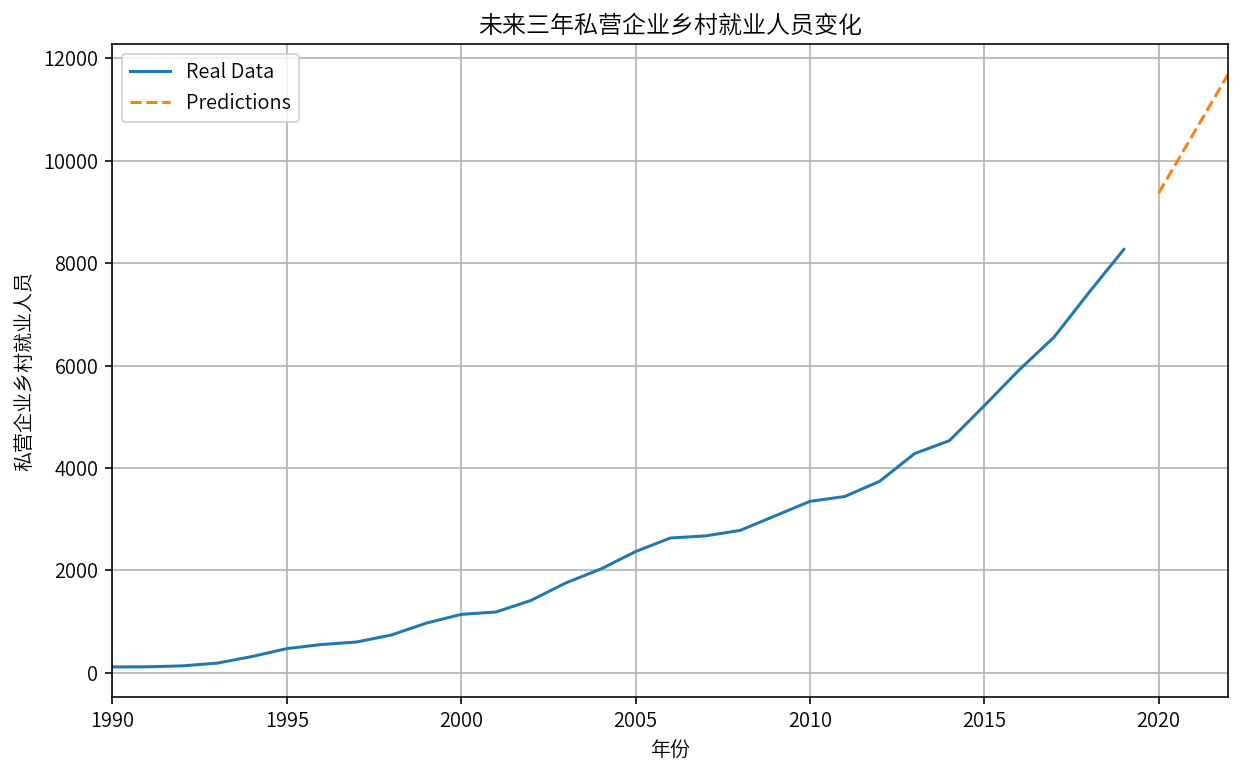
\includegraphics[width=\linewidth]{figures/22.png}
        \caption{未来三年私营企业乡村就业人员变化图}
        \label{fig:prediction_private}
    \end{minipage}\hfill
    \begin{minipage}{0.45\linewidth}
        \centering
        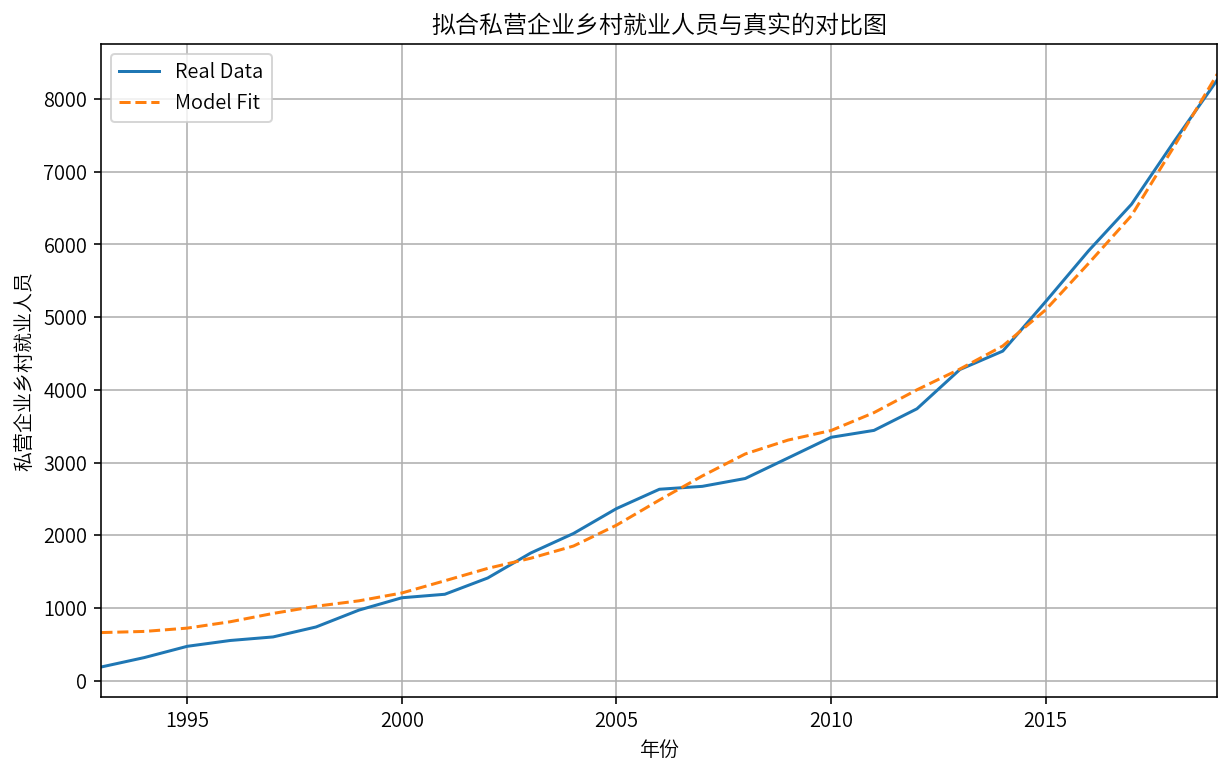
\includegraphics[width=\linewidth]{figures/23.png}
        \caption{拟合私营企业乡村就业人员与真实的对比图}
        \label{fig:fit-vs-real_private}
    \end{minipage}
\end{figure}

根据所呈现的图表分析,可以观察到该模型具有较高的拟合度,并且能够有效地预测趋势。这表明该模型对于描绘乡村私营企业就业人数的变化具有可靠性。利用此模型,成功估算了三年内私营企业乡村就业人员的空缺数据并预测了后三年的结果,详细结果如下表所示。


\begin{table}[H]
\caption{私营企业乡村就业人员数据}
\begin{subtable}{0.5\textwidth}
  \centering
  \caption{补全空缺三年私营企业乡村就业人员}
  \begin{tabular}{cc}
    \hline
    \hline
    \textbf{年份} & \textbf{私营企业乡村就业人员}\\
    \hline
    2020 & 9499.59\\
    2021 & 10732.58\\
    2022 & 12013.71\\
    \hline
  \end{tabular}
\end{subtable}%
\begin{subtable}{0.5\textwidth}
  \centering
  \caption{预测三年私营企业乡村就业人员}
  \begin{tabular}{cc}
    \hline
    \hline
    \textbf{年份} & \textbf{私营企业乡村就业人员}\\
    \hline
    2023 & 13408.71\\
    2024 & 14651.86\\
    2025 & 15764.10\\
    \hline
  \end{tabular}
\end{subtable}

\end{table}


同样地,本文也对个体户乡村就业人员的数据集进行了处理,并生成了相应的图表和数据。

\begin{figure}[H]
    \centering
    \begin{minipage}{0.45\linewidth}
        \centering
        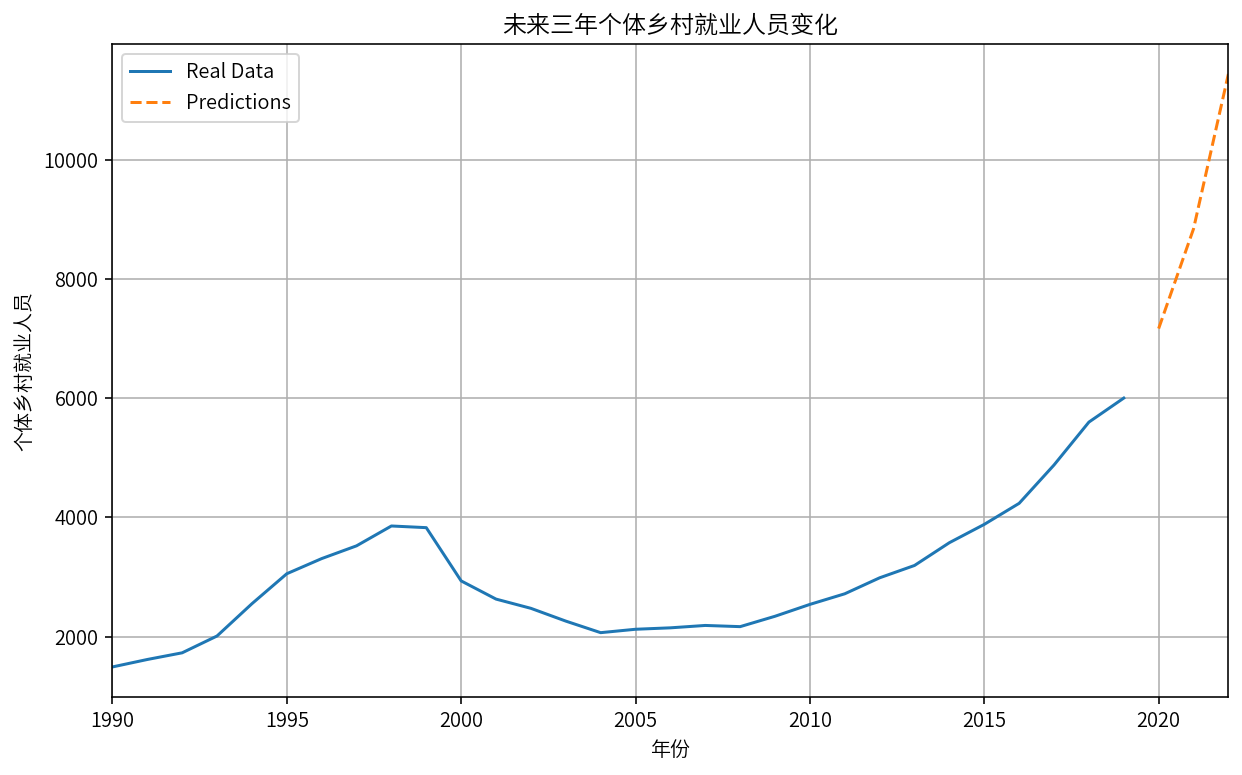
\includegraphics[width=\linewidth]{figures/24.png}
        \caption{未来三年个体户乡村就业人员变化图}
        \label{fig:prediction_self_employed}
    \end{minipage}\hfill
    \begin{minipage}{0.45\linewidth}
        \centering
        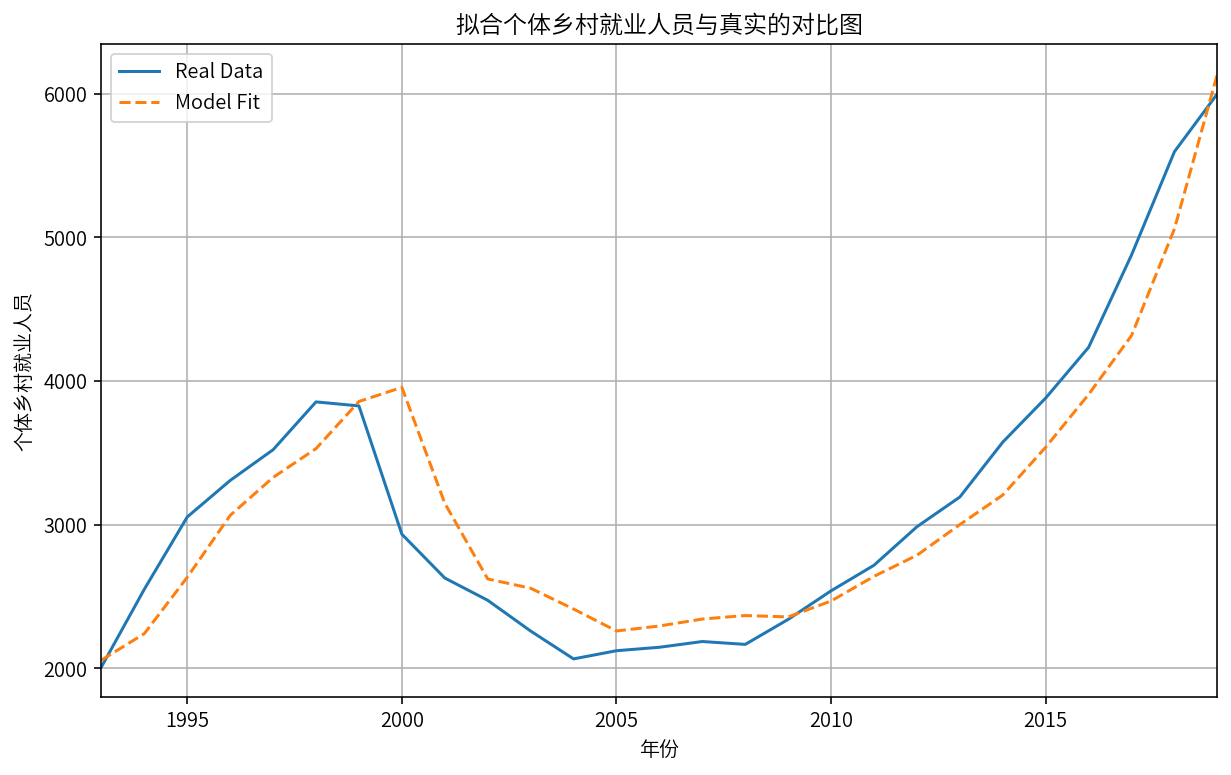
\includegraphics[width=\linewidth]{figures/25.png}
        \caption{拟合个体户乡村就业人员与真实的对比图}
        \label{fig:fit-vs-real_self_employed}
    \end{minipage}
\end{figure}

\begin{table}[H]
\caption{个体户乡村就业人员数据}
\begin{subtable}{0.5\textwidth}
  \centering
  % Table 1
  \caption{补全空缺个体户乡村就业人员}
  \begin{tabular}{cc}
    \hline
    \hline
    \textbf{年份} & \textbf{个体户乡村就业人员}\\
    \hline
    2020 & 7228.06\\
    2021 & 8956.09\\
    2022 & 11552.06\\
    \hline
  \end{tabular}
\end{subtable}%
\begin{subtable}{0.5\textwidth}
  \centering
  % Table 2
  \caption{预测后三年个体户乡村就业人员}
  \begin{tabular}{cc}
    \hline
    \hline
    \textbf{年份} & \textbf{个体户乡村就业人员}\\
    \hline
    2023 & 14889.481\\
    2024 & 17813.33\\
    2025 & 19633.70\\
    \hline
  \end{tabular}
\end{subtable}

\end{table}

据数据预测,个体户乡村就业人员和私营企业乡村就业人员将继续实现较大增长。这表明,农业就业的核心理论正在从传统范式转变为以个体户和私营企业为主导。

采用与前述相同的方法,本文利用DLF-LSTM模型对城乡就业人员数据进行了预测。经过模型的训练与验证,得到了预测未来十年城乡就业人数变化的图表和数据。

\begin{figure}[h]
    \centering
    \begin{minipage}{0.3\linewidth}
        \centering
        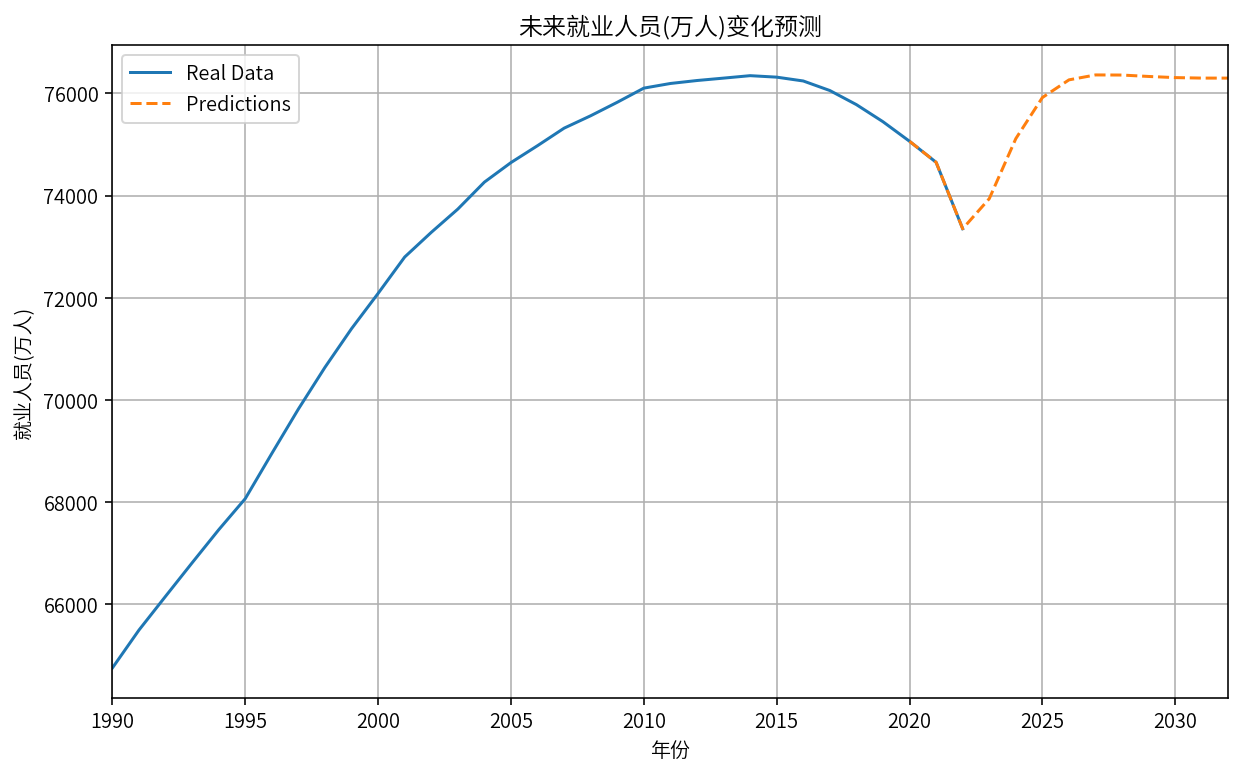
\includegraphics[width=\linewidth]{figures/26.png}
        \caption{未来就业人员变化预测}
        \label{fig:prediction_employment}
    \end{minipage}\hfill
    \begin{minipage}{0.3\linewidth}
        \centering
        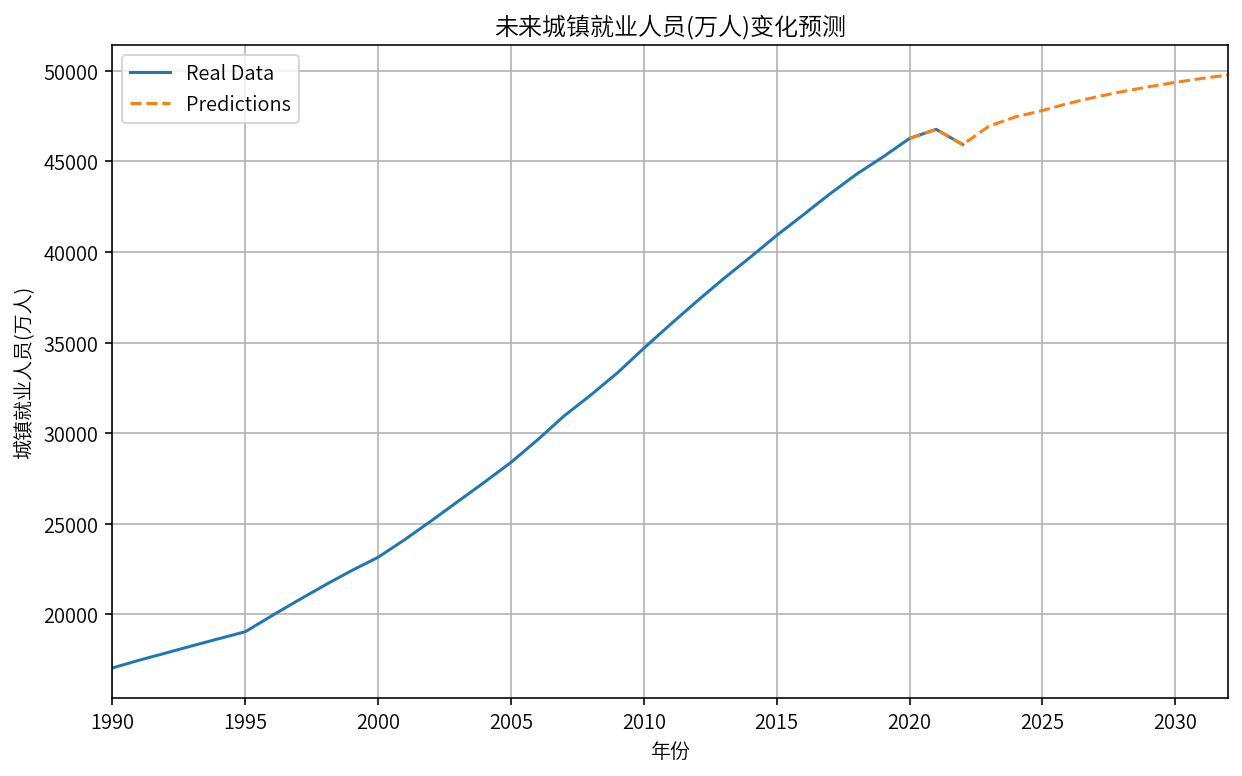
\includegraphics[width=\linewidth]{figures/27.png}
        \caption{城镇就业人员变化预测}
        \label{fig:fit-vs-real_employment_city}
    \end{minipage}\hfill
    \begin{minipage}{0.3\linewidth}
        \centering
        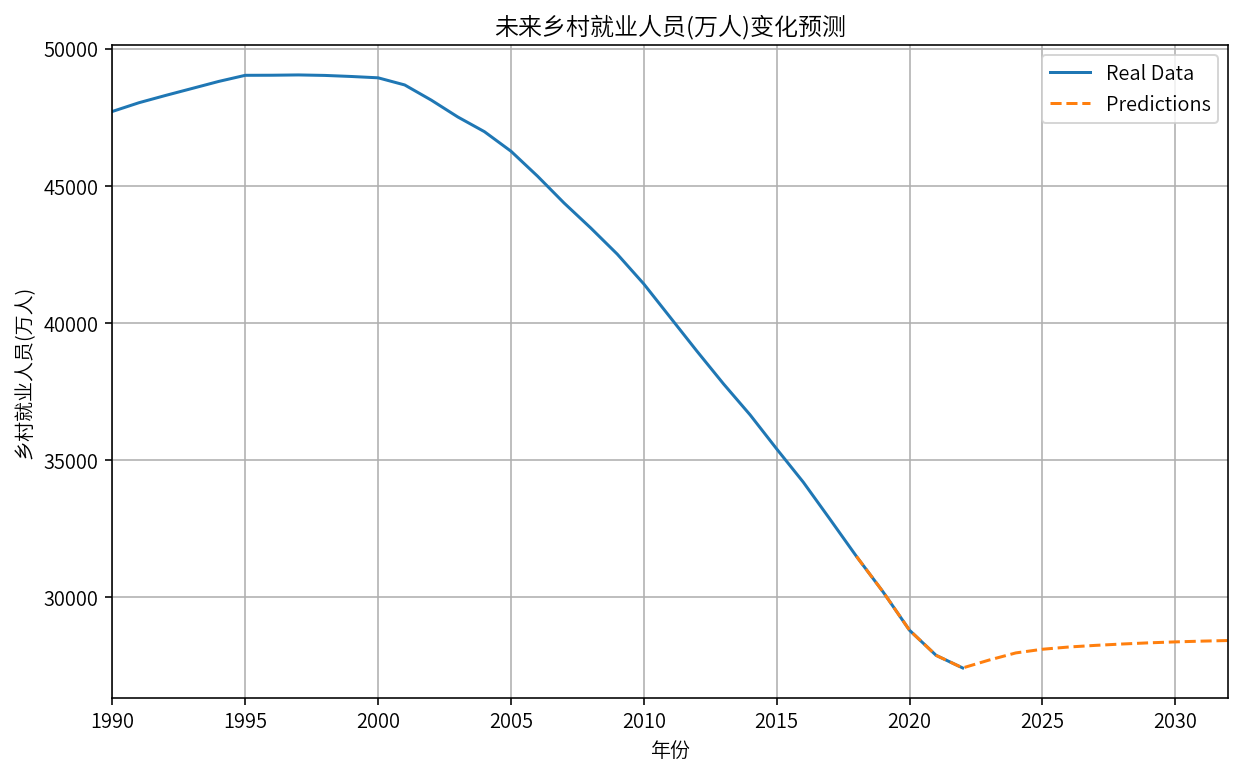
\includegraphics[width=\linewidth]{figures/28.png}
        \caption{乡村就业人员变化预测}
        \label{fig:fit-vs-real_employment_village}
    \end{minipage}
\end{figure}

图表显示总就业人数在经历了一个上升趋势之后,趋于平稳并略有波动。预测显示未来会有一定的波动,但总体维持在一个相对平稳的水平。这可能意味着就业市场在达到一定规模后,将进入一个较为成熟的阶段,增长速度放缓。

预计城镇就业人员数量将继续呈现上升趋势,不过增长速度逐渐放缓,显示出一个逐渐稳定的趋势。这表明城镇就业市场的发展已经逐渐趋向成熟,未来的增长可能更多地受到经济周期和政策调控的影响。

\begin{table}[h]
    \centering
    \begin{minipage}{0.32\linewidth}
        \centering
        \caption{预测就业人员变化}
        \label{tab:total_employment}
        \begin{tabular}{cc}
        \hline
        年份 & 预测就业人员(万人) \\
        \hline
        2020 & 73939.57 \\
        2021 & 75116.24 \\
        2022 & 75921.16 \\
        2023 & 76266.91 \\
        \hline
        \end{tabular}
    \end{minipage}\hfill
    \begin{minipage}{0.32\linewidth}
        \centering
        \caption{城镇就业人员变化预测}
        \label{tab:urban_employment}
        \begin{tabular}{cc}
        \hline
        年份 & 预测城镇就业人员(万人) \\
        \hline
        2020 & 46958.44 \\
        2021 & 47466.87 \\
        2022 & 47811.33 \\
        2023 & 48213.55 \\
        \hline
        \end{tabular}
    \end{minipage}\hfill
    \begin{minipage}{0.32\linewidth}
        \centering
        \caption{乡村就业人员变化预测}
        \label{tab:rural_employment}
        \begin{tabular}{cc}
        \hline
        年份 & 预测乡村就业人员(万人) \\
        \hline
        2018 & 27709.54 \\
        2019 & 27967.95 \\
        2020 & 28101.58 \\
        2021 & 28183.98 \\
        \hline
        \end{tabular}
    \end{minipage}
\end{table}


农村就业人员数的预测在初始阶段显示下降趋势,随后转为平稳甚至上升趋势。这可能反映了随着农业自动化和工业化的推进,农村劳动力需求减少,但随着政策支持和农村经济结构的逐步调整,农村就业人数将趋于稳定,或呈现增长趋势。

\section{可支配收入}
农民生活水平的提升建立在农民可支配收入的基础上,可支配收入直接影响到农民的消费能力。只有当农民拥有足够的可支配收入时,他们才能够改善自身及家庭的生活质量,满足日益增长的物质和文化需求,进而推动农村社会的整体进步与繁荣。

% 本文收集了2016年至2023年期间的农民可支配收入数据,以此为基础绘制了相应的折线图,如下图所示:

% \begin{figure}[h]
%     \centering
%     \begin{subfigure}{0.5\textwidth}
%         \centering
%         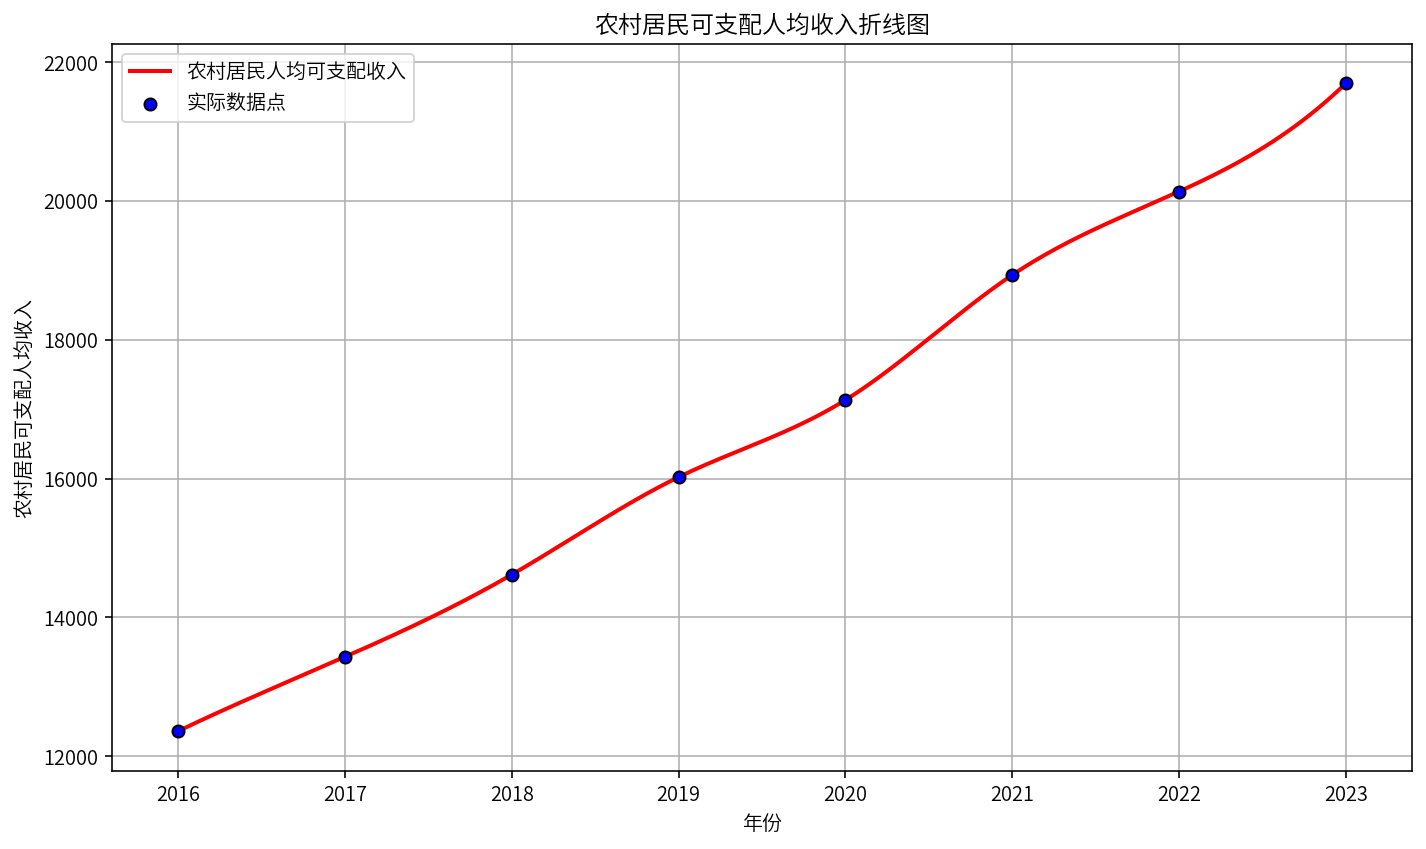
\includegraphics[width=\linewidth]{figures/39.png}
%         \caption{农村可支配收入折线图}
%         \label{fig:sub1}
%     \end{subfigure}%
%     \begin{subfigure}{0.5\textwidth}
%         \centering
%         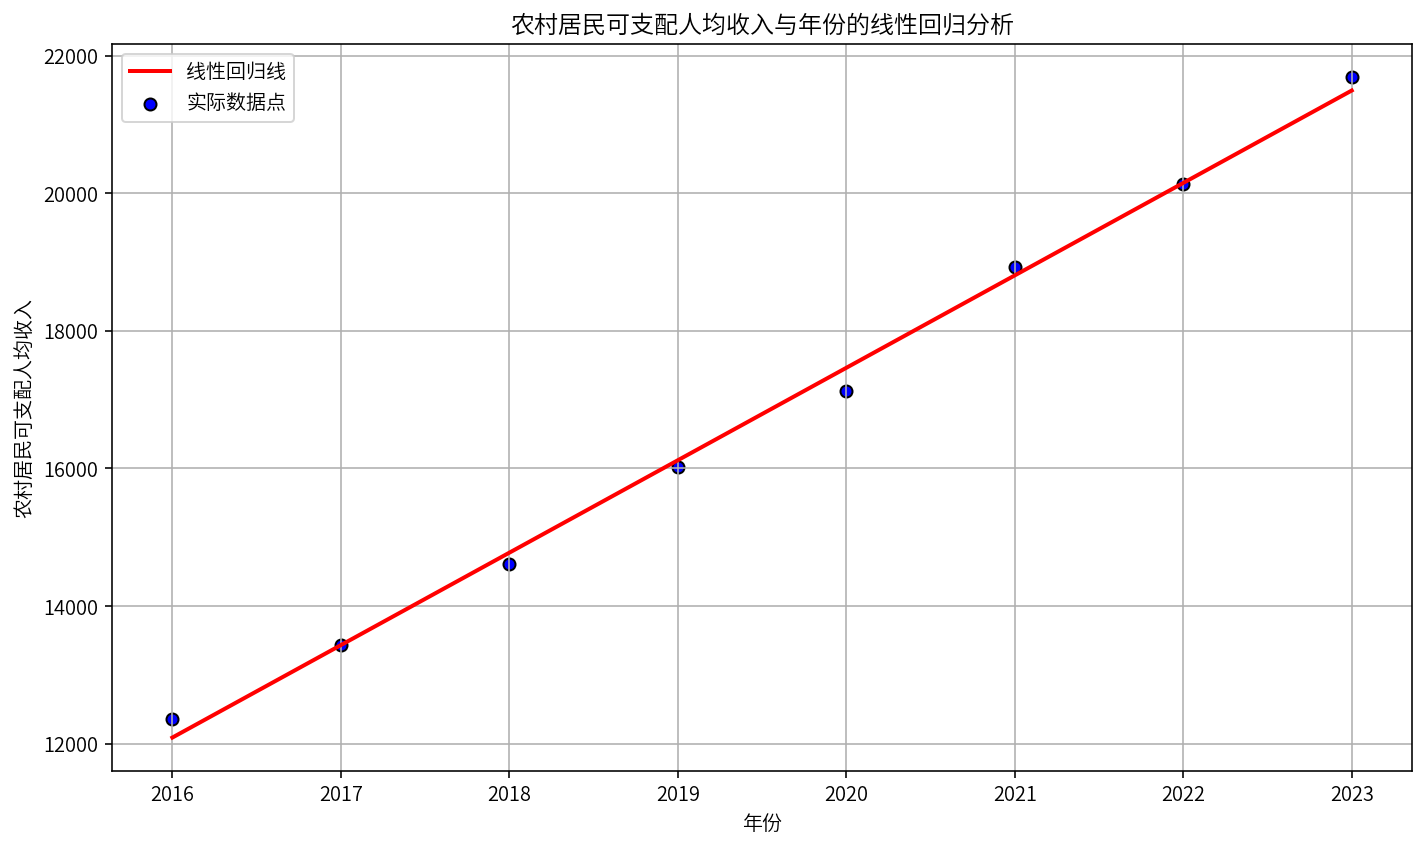
\includegraphics[width=\linewidth]{figures/38.png}
%         \caption{农村可支配收入拟合线性图}
%         \label{fig:sub2}
%     \end{subfigure}
%     \caption{农村可支配收入图}
%     \label{fig:combined}
% \end{figure}


% 图5.9清楚显示,农民的可支配收入逐年稳定增长,并且增速有加快的迹象。整体呈现出线性趋势。这种连续且一致的上升趋势,没有显著波动或下跌的现象,表明在过去几年中,农民的经济状况稳定向好。这不仅预示着农民生活水平的普遍提升,也反映了农村经济发展政策可能的正面效果。

本文详细汇编并分析了从1999年至2022年间,中国农村地区居民的可支配收入与消费支出的全面数据集。研究的核心在于运用斯皮尔曼等级相关系数这一强有力的非参数统计工具,该方法无需假设数据服从特定分布,即可有效评估两个变量间是否存在单调递增或递减的关系。
通过计算如下公式
\begin{equation}
\rho = 1 - \frac{6 \sum d_i^2}{n(n^2 - 1)}
\hspace{1em}
\footnote{其中 \(\rho\) 表征相关程度,\(d_i\) 为每一对观测值在各自排序后之差,而 \(n\) 代表样本总量}
\end{equation}

我们深入探讨了收入与支出变量间潜在的关联模式。分析结果显示,相关性图表清晰地揭示了农村居民可支配收入与其消费支出之间存在极为紧密且显著的相关性趋势。
\begin{figure}[H]
    \centering
    \begin{subfigure}{0.5\textwidth}
        \centering
        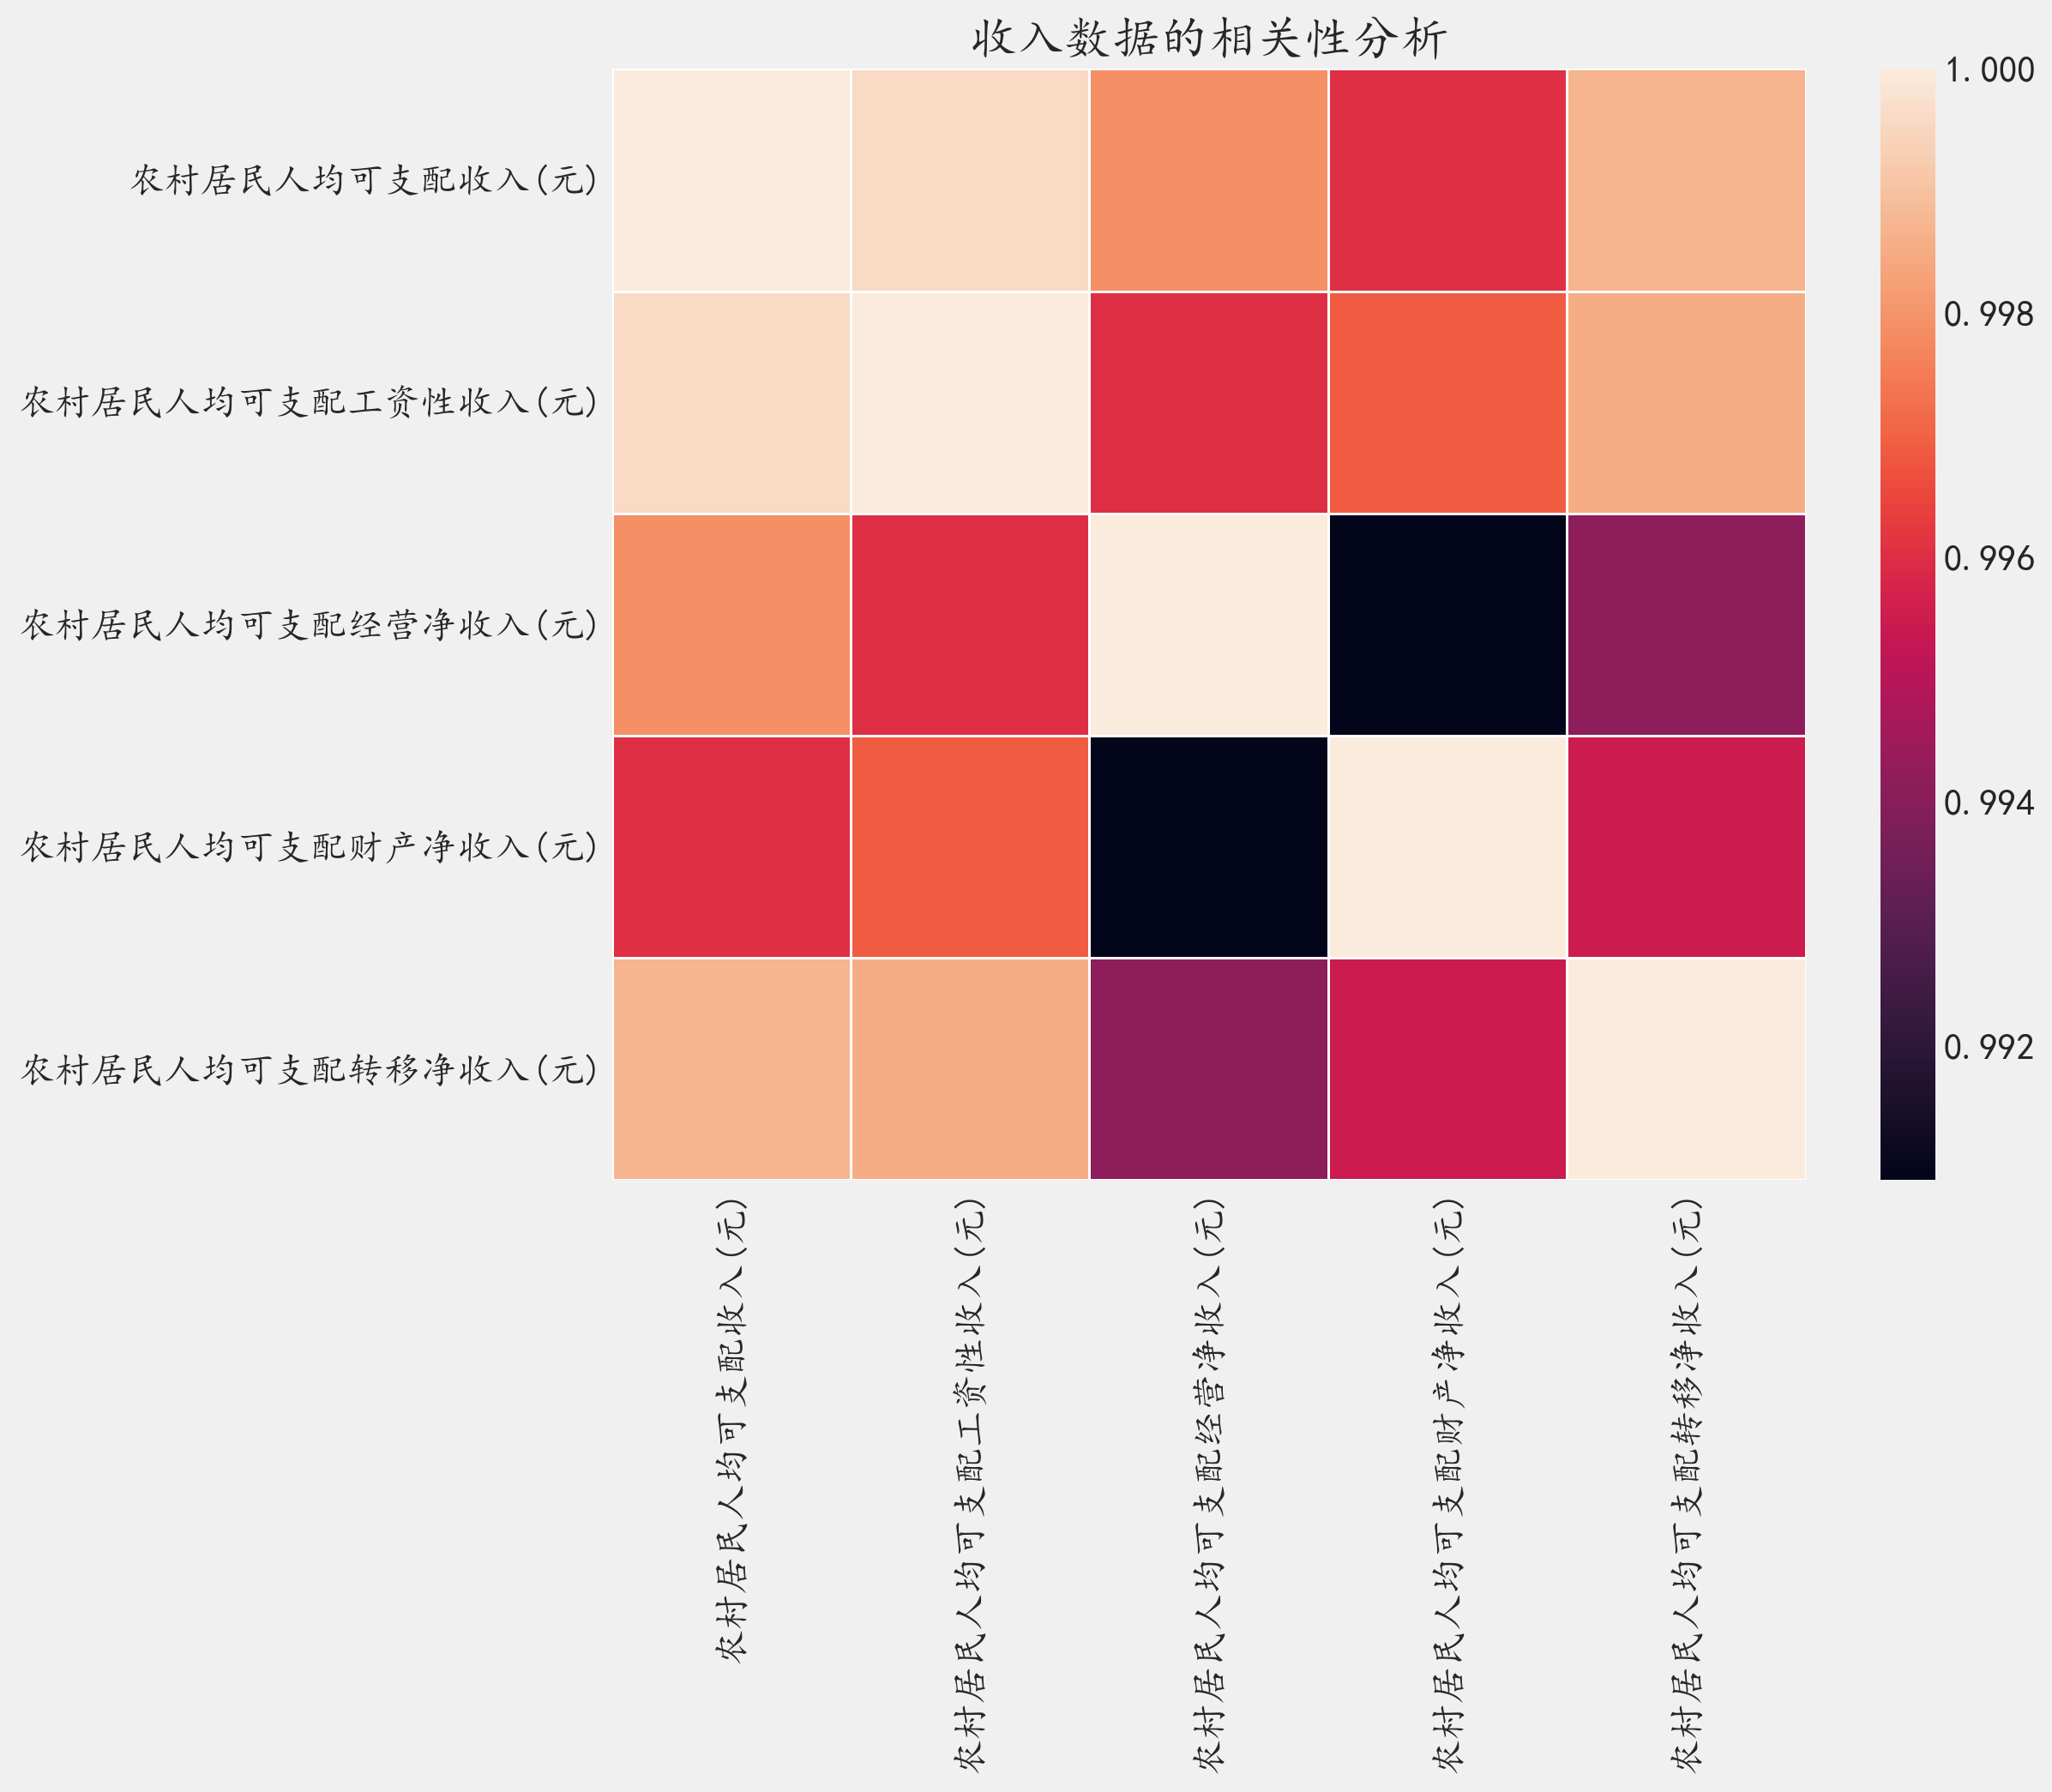
\includegraphics[width=\linewidth]{figures/income_corr.png}
        \caption{收入数据的相关性分析}
        \label{fig:income_corr}
    \end{subfigure}
    \begin{subfigure}{0.49\textwidth}
        \centering
        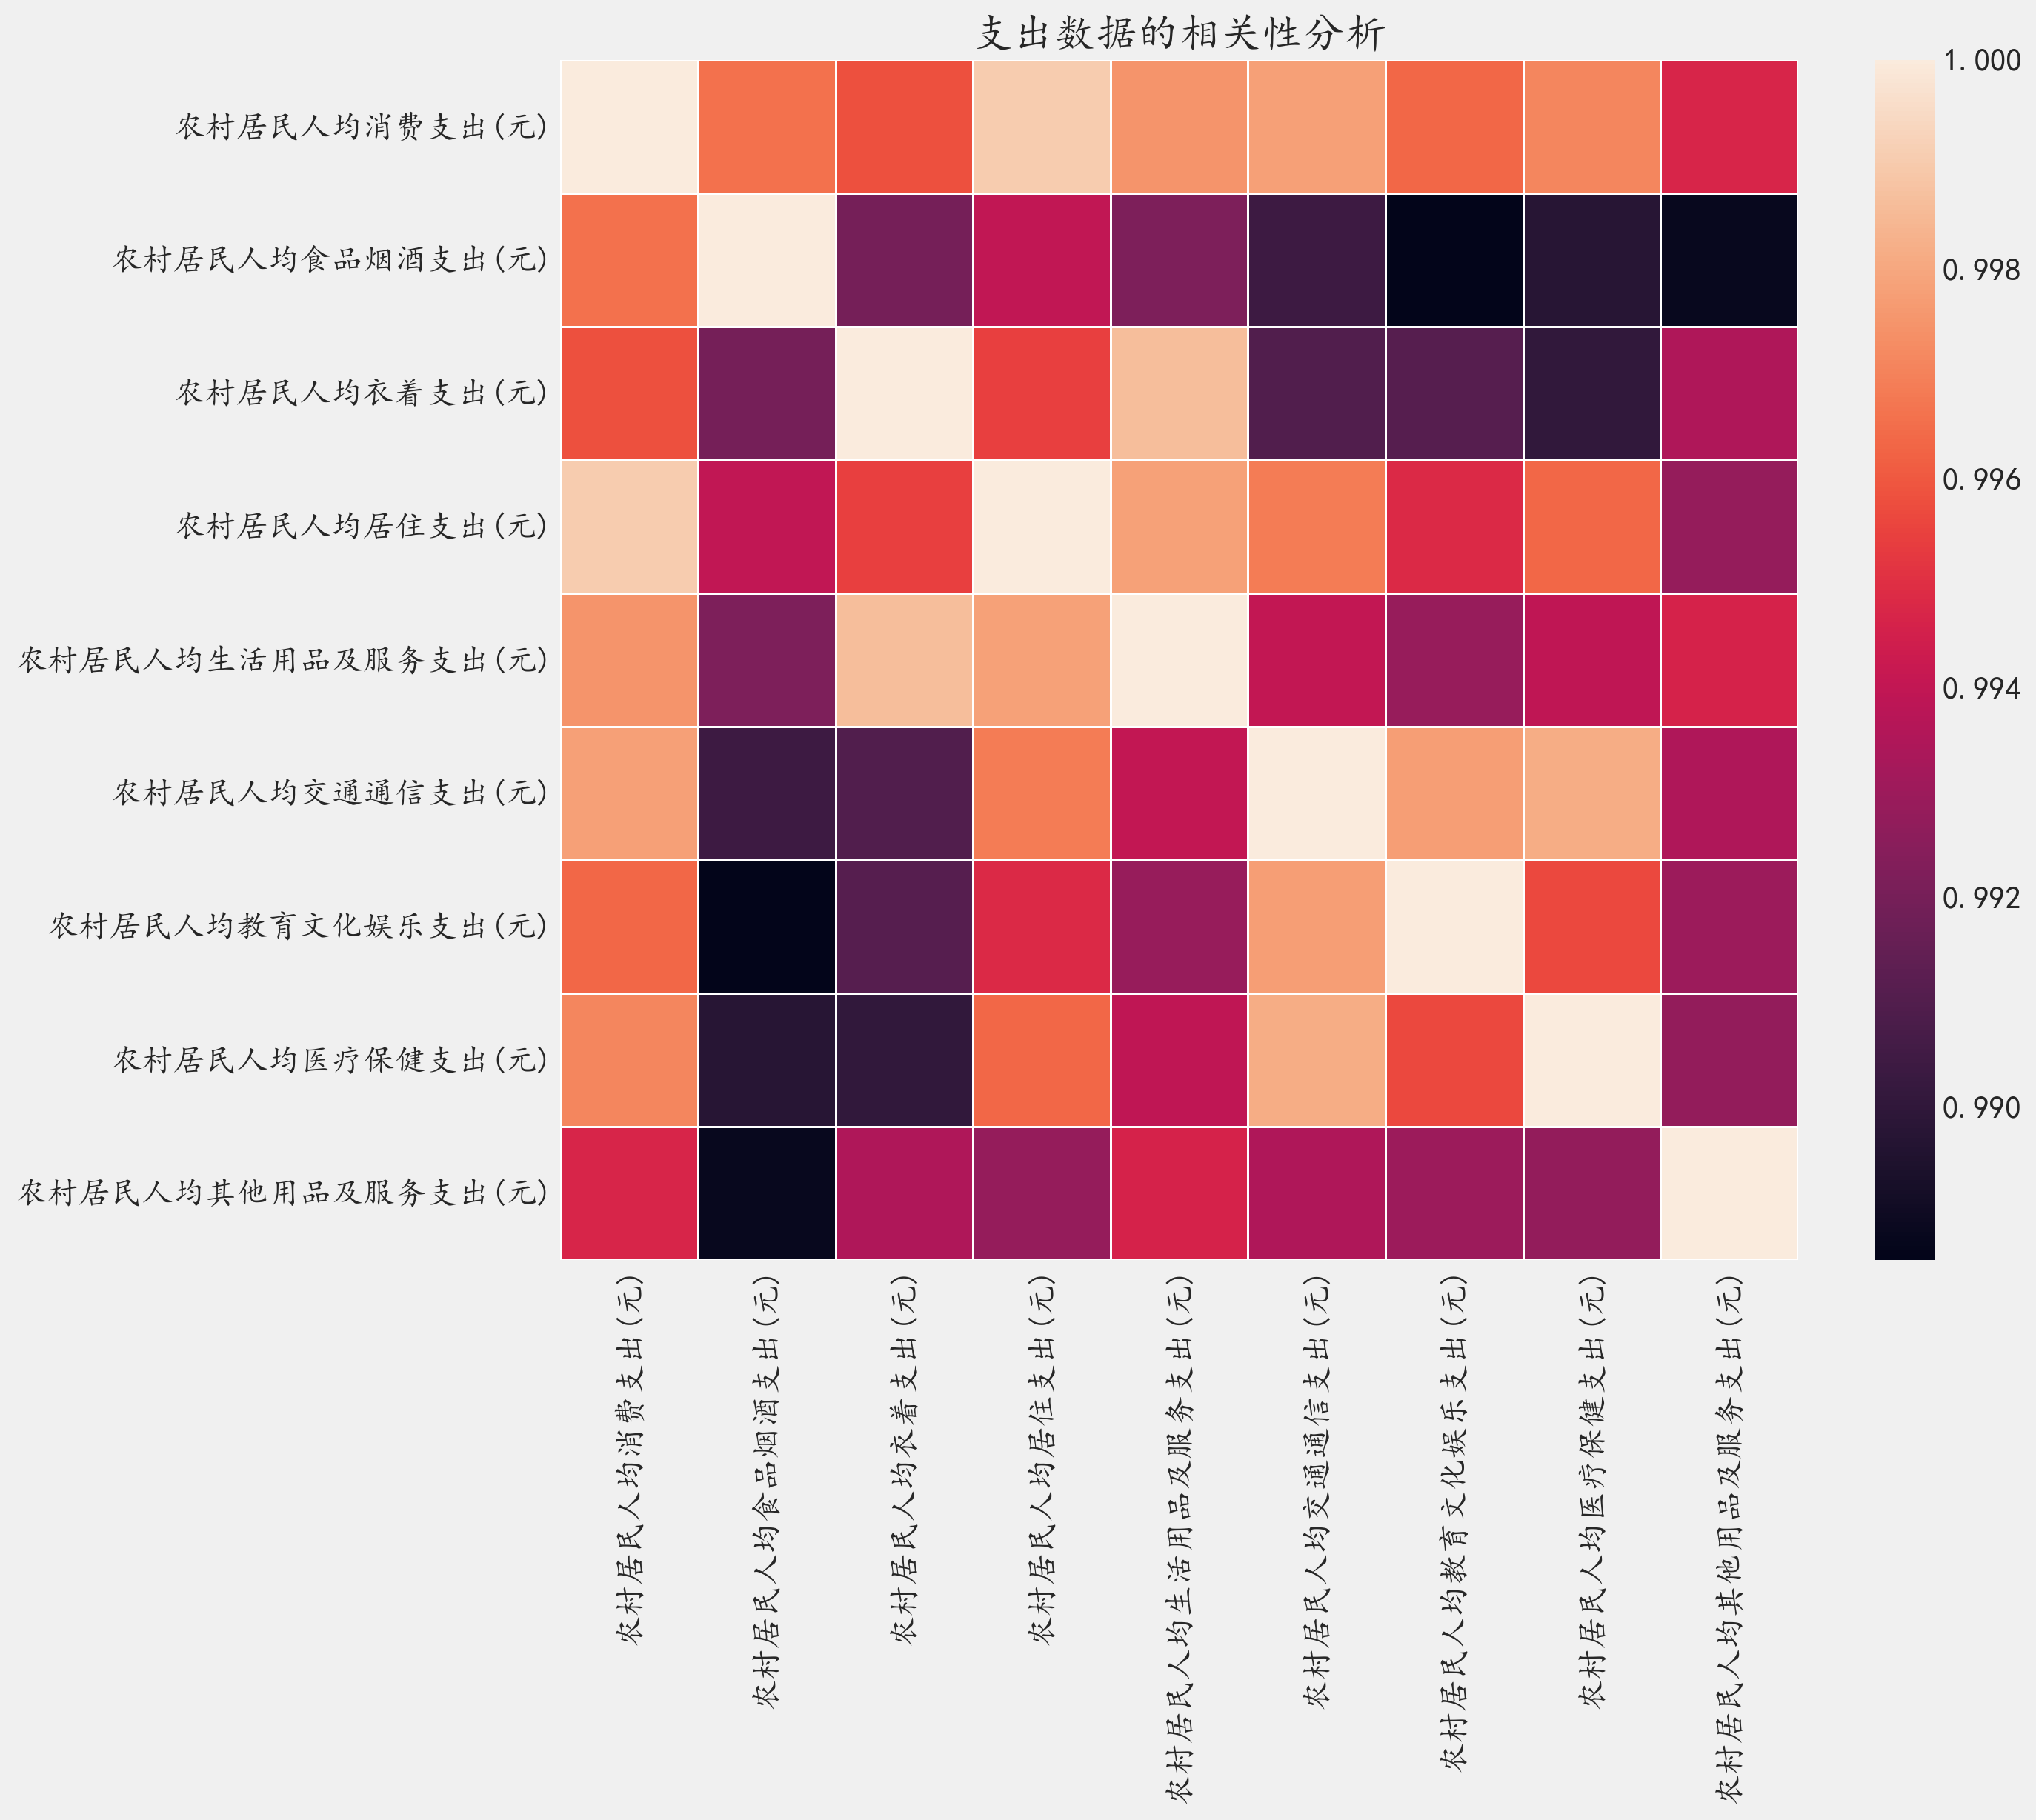
\includegraphics[width=\linewidth]{figures/expenditure_corr.png}
        \caption{支出数据的相关性分析}
        \label{fig:expenditure_corr}
    \end{subfigure}
    \caption{斯皮尔曼等级相关系数分析图表}
\end{figure}

为进一步深化理解,本研究采取了主成分分析(PCA)技术,这是一种强大的降维手段,旨在从复杂的数据集中提炼出最具解释力的综合指标。PCA通过将原始变量转换到新的坐标系统中,即主成分方向上,以最能解释数据方差的方式重新表达数据,其结果不仅依赖于数据自身的属性,还与预处理步骤如数据的中心化和标准化密切相关。所获得的PCA图表生动展现了收入与支出数据在新维度上的结构特征,有助于揭示隐藏的模式和减少冗余信息。

\begin{figure}[H]
    \centering
    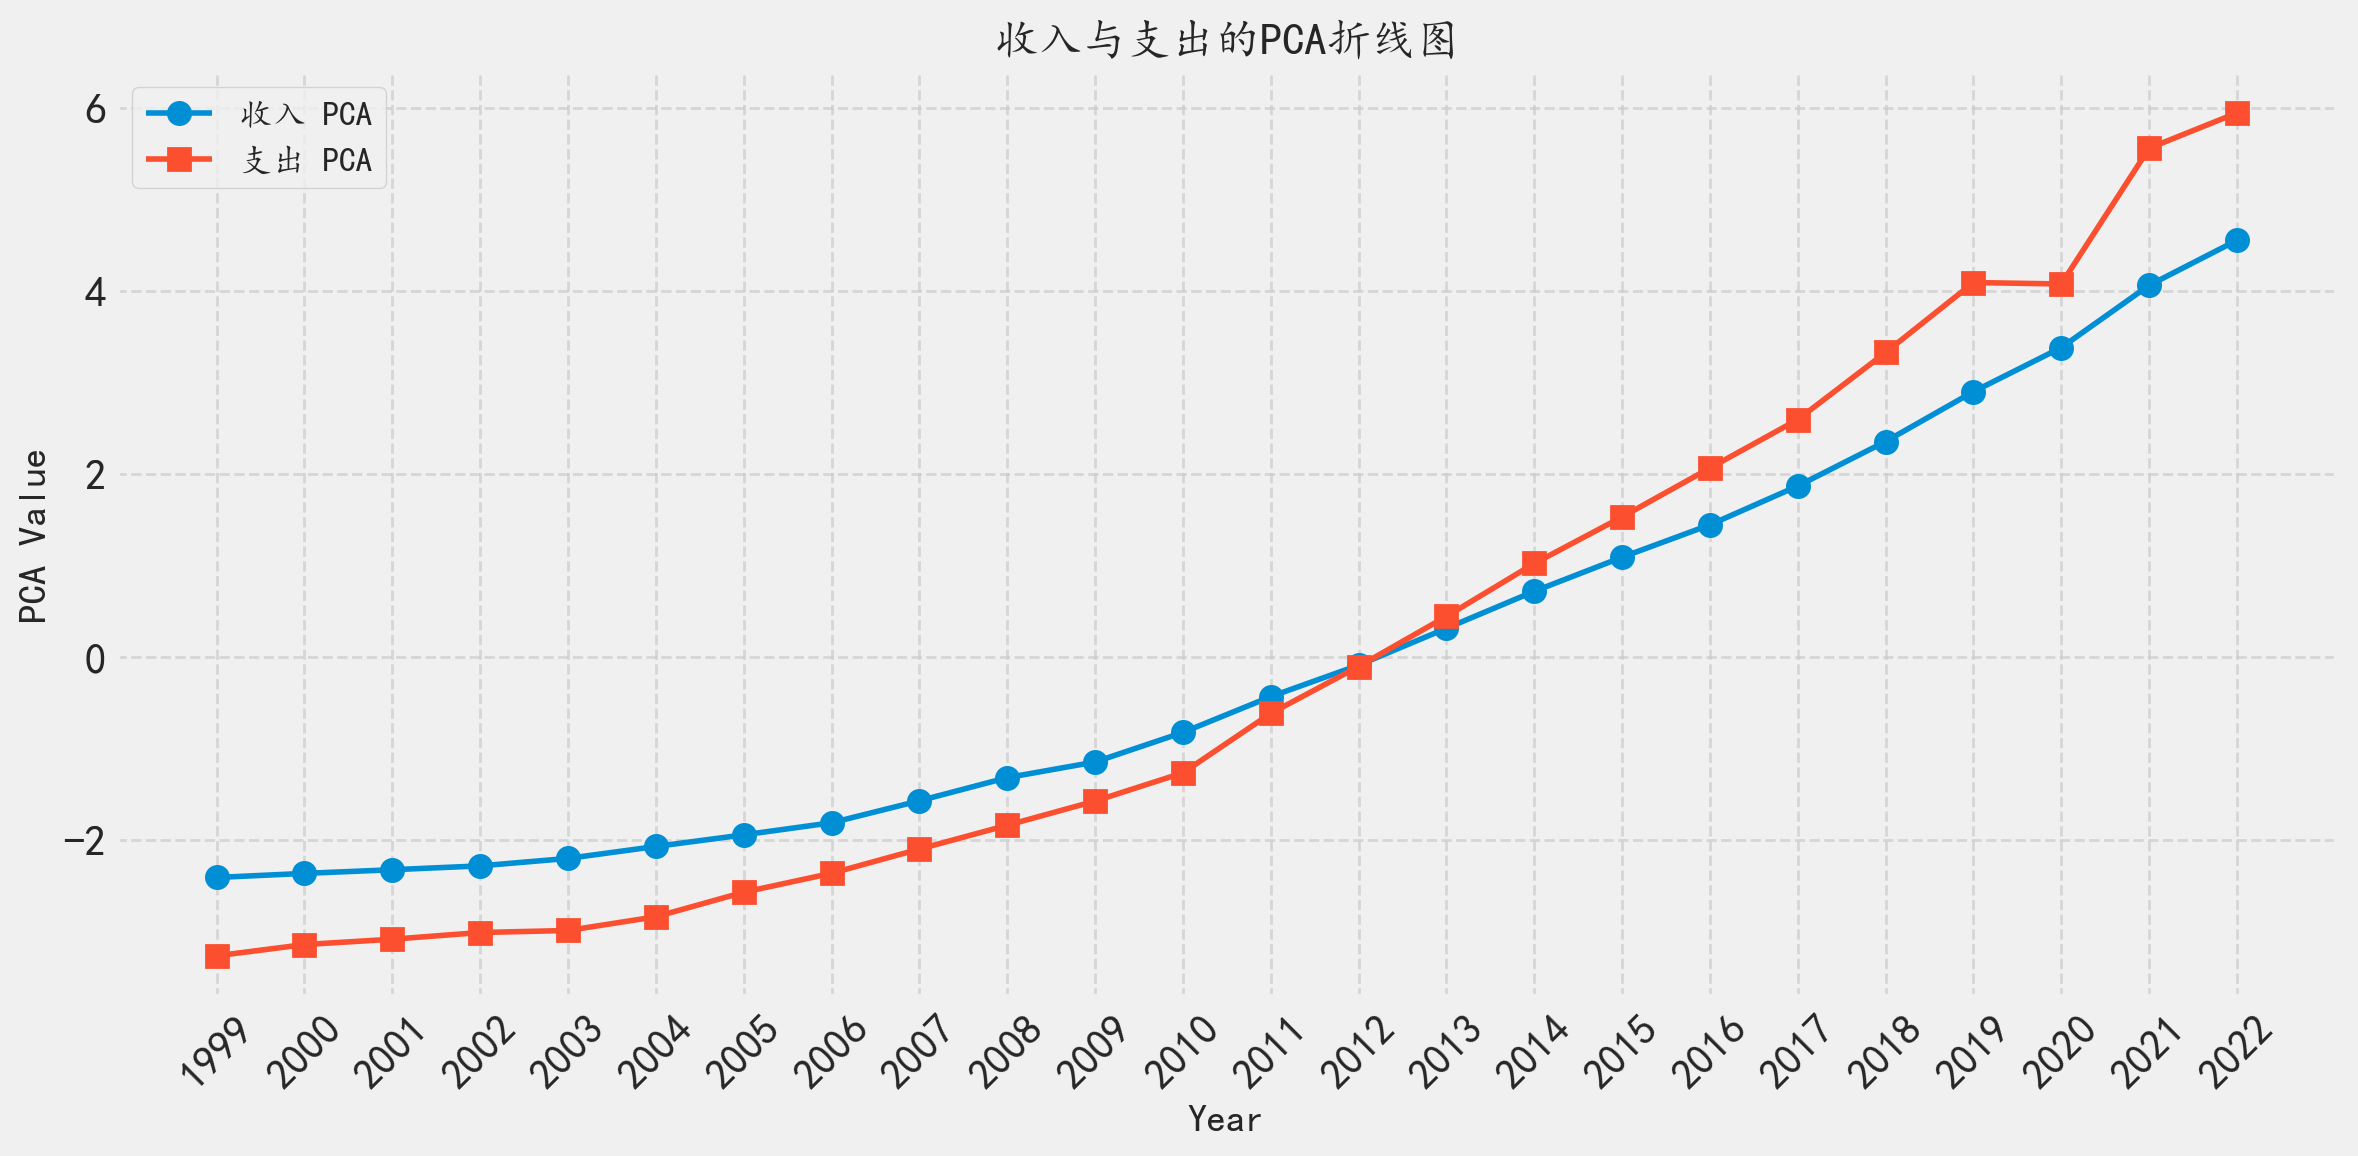
\includegraphics[width=0.75\linewidth]{figures/PCA.png}
    \caption{主成分分析图表}
    \label{fig:PCA}
\end{figure}

在此基础上,我们采用牛顿多元法执行非线性回归分析,以模型 \(a * x^2 + b * x + c\) 描述农村居民收入与消费支出随时间变化的动态规律,成功拟合了数据曲线。这一发现不仅加深了我们对农村经济活动周期性和长期趋势的理解,也为政策制定者提供了宝贵的量化依据。

\begin{figure}[H]
    \centering
    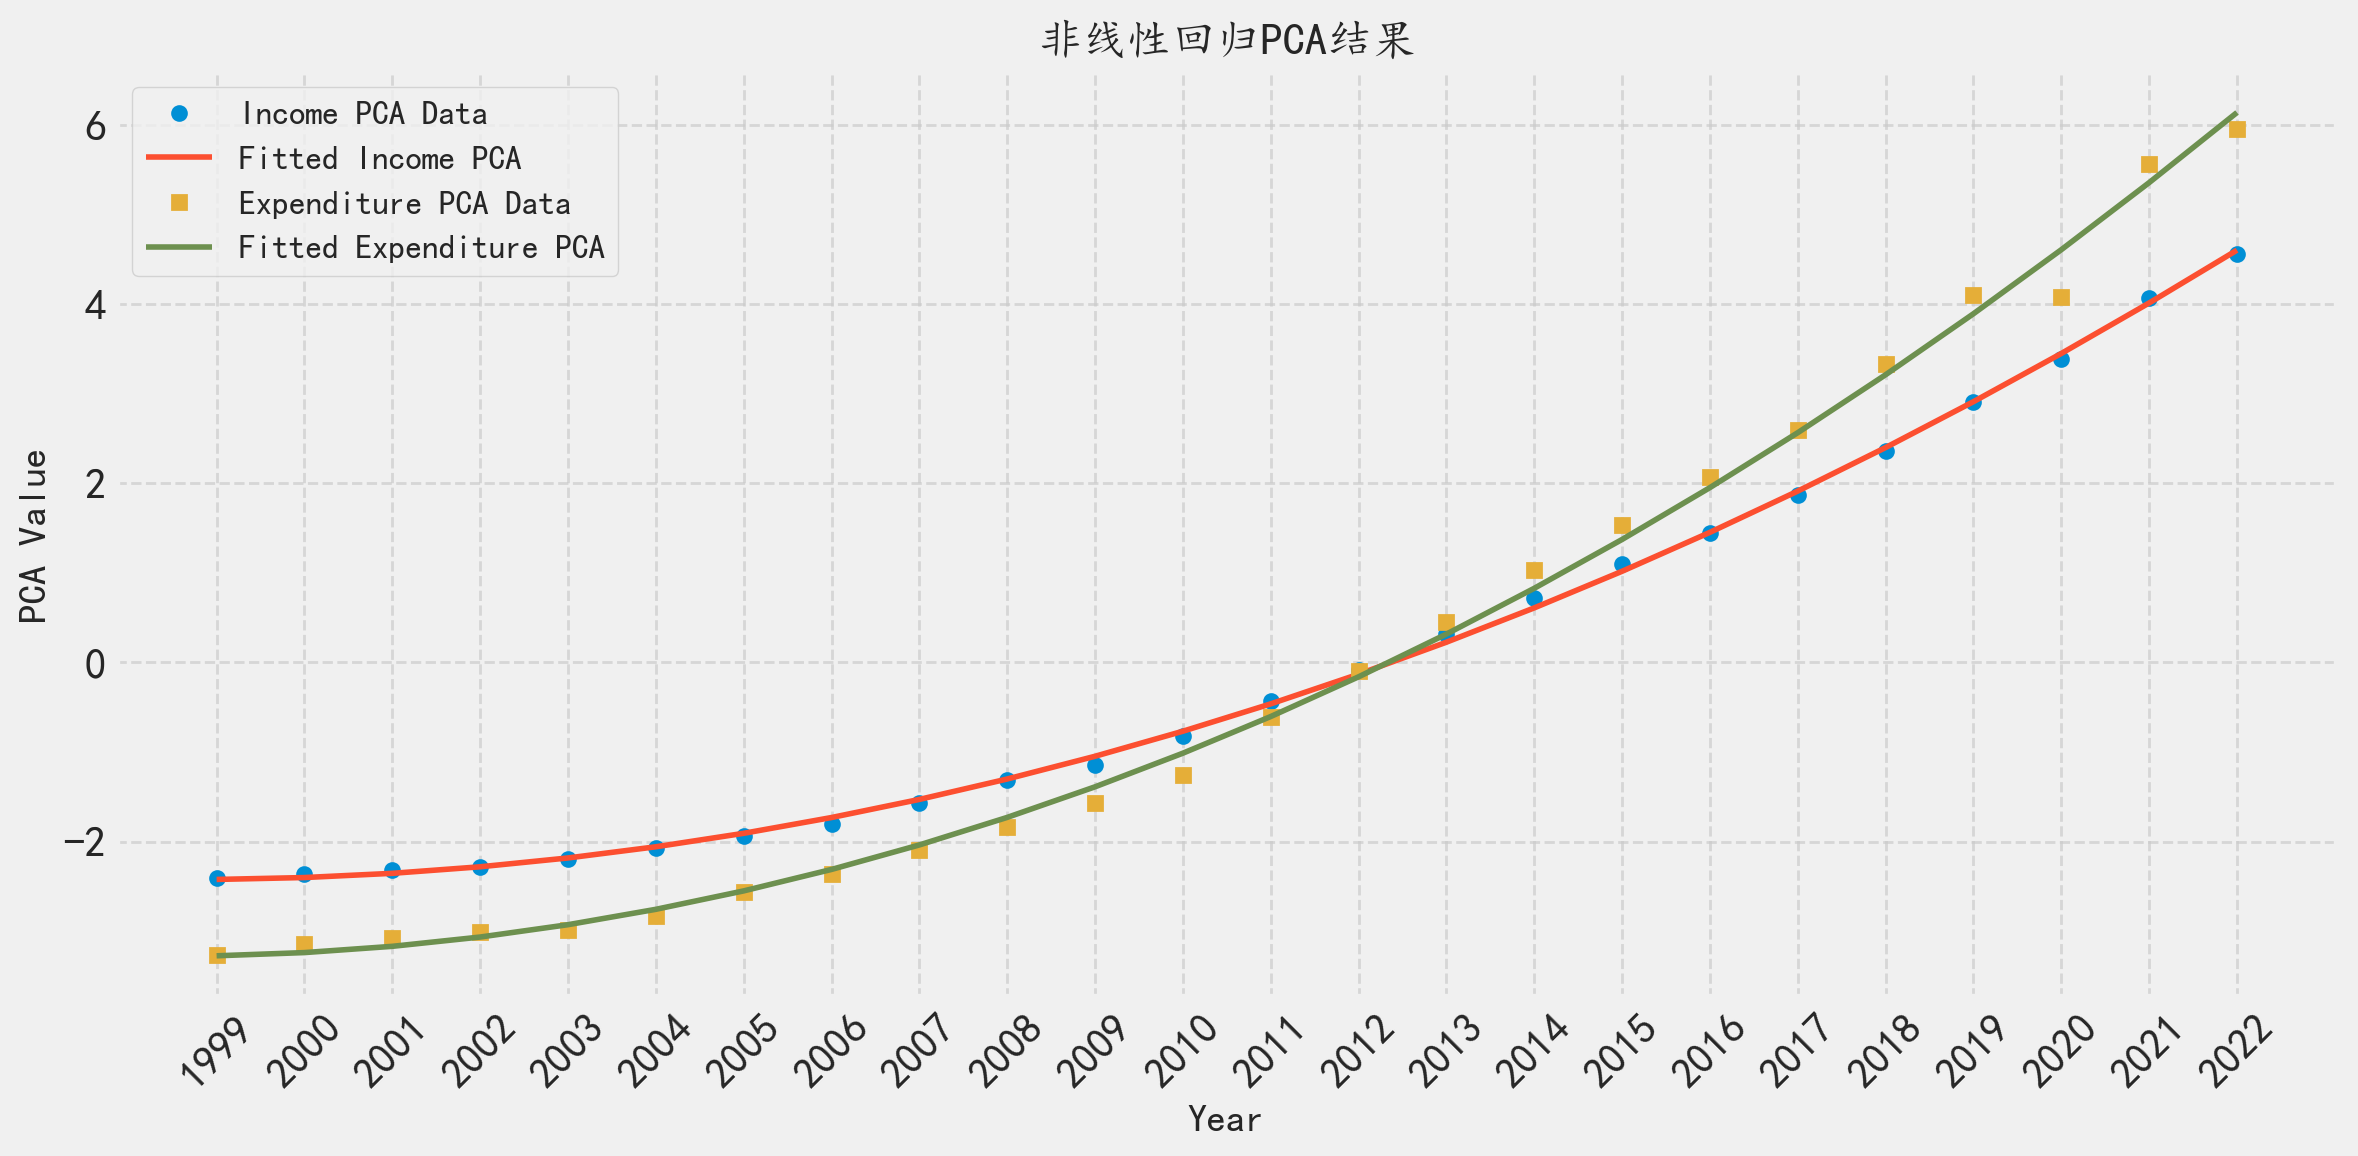
\includegraphics[width=0.75\linewidth]{figures/poly_PCA.png}
    \caption{非线性回归PCA结果}
    \label{fig:poly_PCA}
\end{figure}

最后,通过对比平均收入与平均消费支出的年度折线图,研究揭示了一个令人关注的趋势:两者间的差距随着时间推移而逐渐扩大,这凸显了农村经济发展中人民生活愈加富裕,表现了制定精准有效的政策措施,促进农村经济的均衡发展和提升农村居民的生活水平获得卓越成效。

\begin{figure}[H]
    \centering
    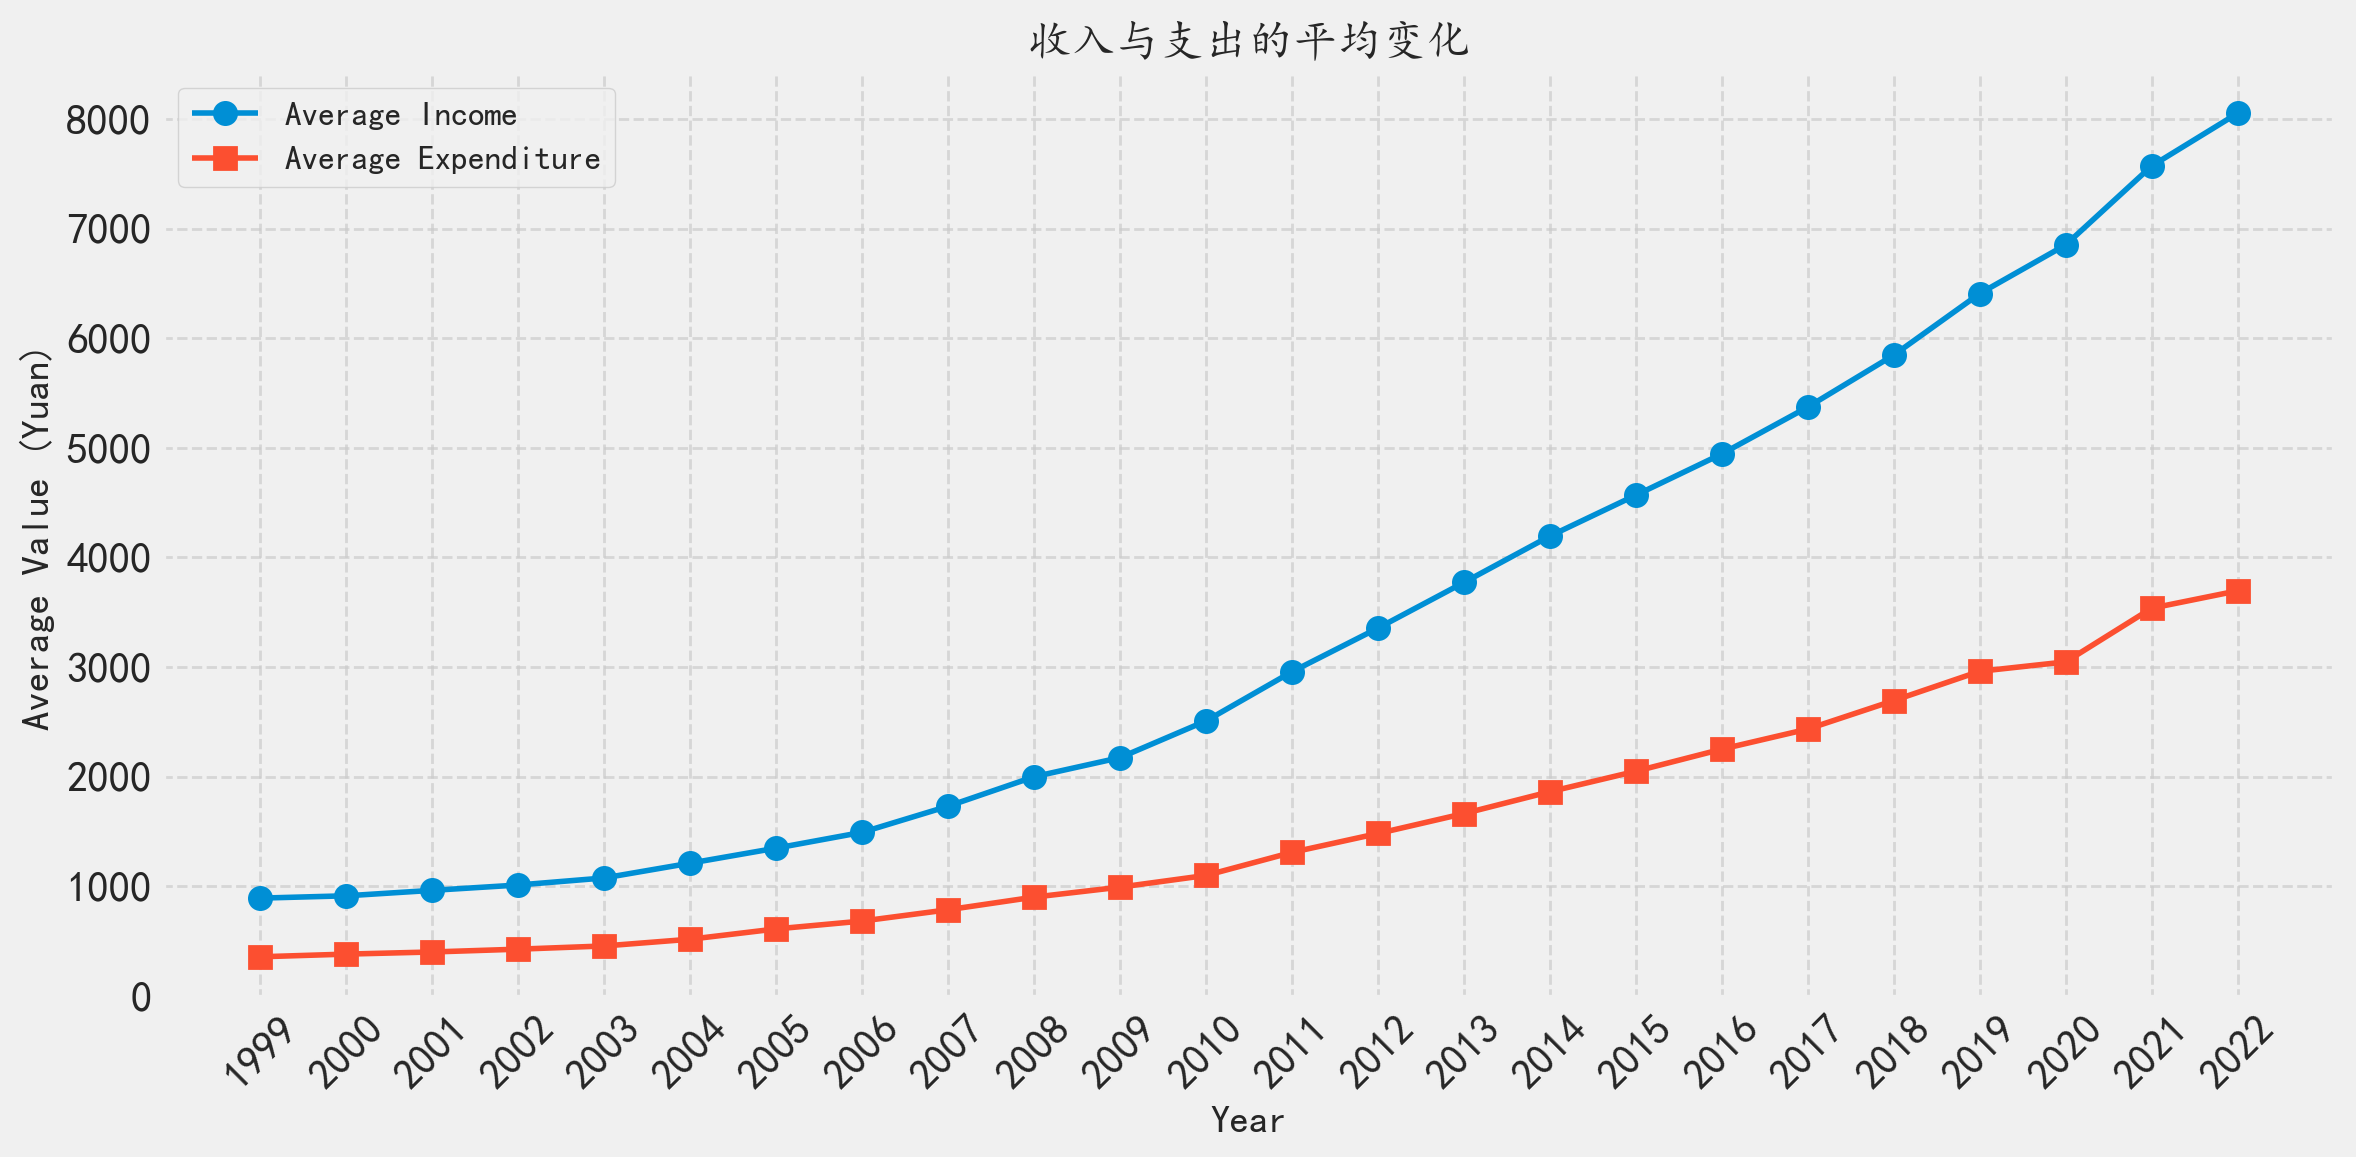
\includegraphics[width=0.75\linewidth]{figures/average_change.png}
    \caption{收入支出平均年化折线图}
    \label{fig:average_change}
\end{figure}

\section{基本生活}

在诸多因素如可支配收入的增加、科技的迅速进步以及政策的积极推动下,乡村居民的生活质量无疑正处于不断提升的轨迹之上。为了深入分析这一变化,我们采集并利用了关于主要交通工具和基础家用电器的拥有量数据,对比了过去十年与当前情况下的数据绘制了雷达图:

\begin{figure}[H]
    \centering
    \begin{minipage}{0.43\textwidth}
        \centering
        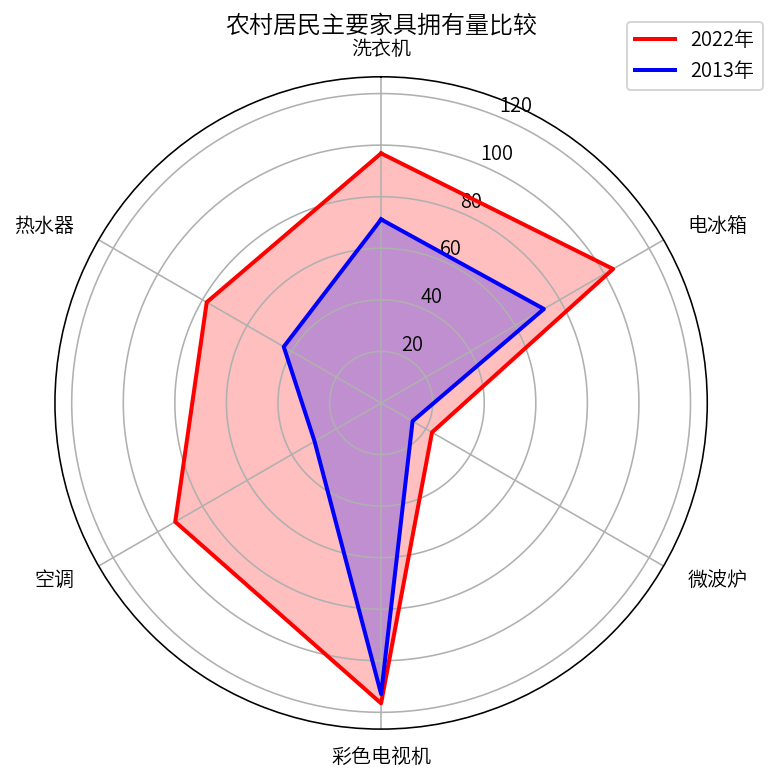
\includegraphics[width=\linewidth]{figures/43.png}
        \caption{农村居民主要家具拥有量比较}
        \label{fig:furniture}
    \end{minipage}\hfill
    \begin{minipage}{0.43\textwidth}
        \centering
        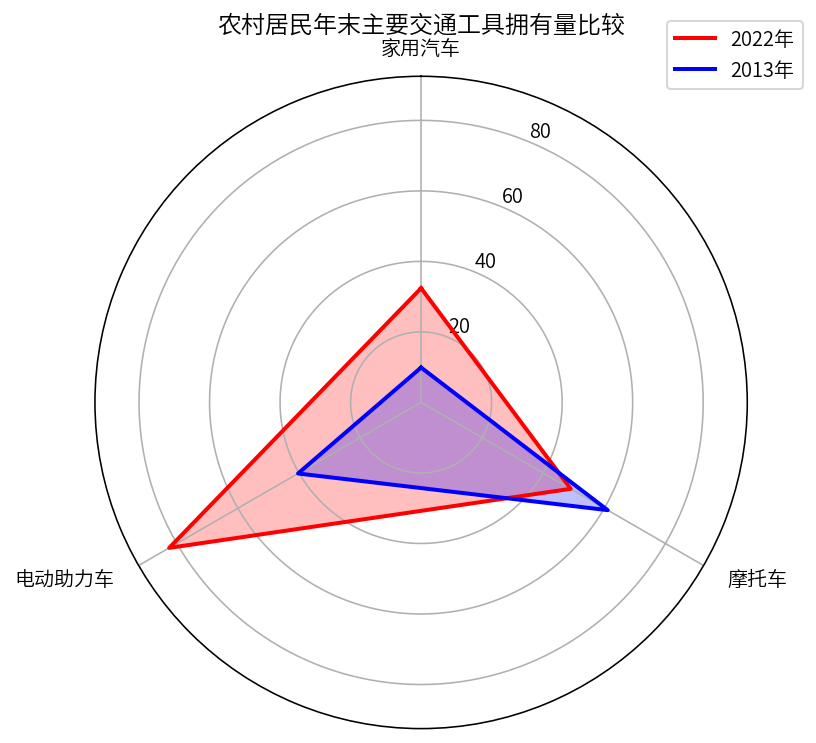
\includegraphics[width=\linewidth]{figures/44.png}
        \caption{农村居民年末主要交通工具拥有量比较}
        \label{fig:vehicles}
    \end{minipage}
\end{figure}


通过细致构建的雷达图,得以直接洞察到洗衣机、电冰箱、微波炉、彩色电视机、空调以及热水器等基础家电的拥有量显著增加,这一变化凸显了乡村居民生活水平的提升和生活质量的改善。交通工具中,除摩托车受到政策变动的影响出现了下降趋势,家用汽车和电动助力车实现了显著增长,这不仅反映了乡村地区交通工具使用模式的变化,也突显了现代化进程中对于便捷交通方式的日益增长需求。

\section{幸福指数}

根据马斯洛需求层次理论,人的需求从低到高分为生理需求、安全需求、社会需求、尊重需求和自我实现需求。生活水平的提升不应局限于物质层面的丰富,更应包括精神层面的满足。

其中,恩格尔系数,即家庭食品支出占总消费支出的比重,是反映居民生活水平的重要经济指标。该系数越低,表明家庭在食品上的支出占比越小,一般而言,家庭的生活水平越高。

本文搜集了自改革开放以来至今的全国居民(包括城镇和乡村居民)的恩格尔系数数据\cite{china-engel-coefficients},并据此绘制了反映全国总体以及农村居民恩格尔系数变化的折线图,如下图所示。

\begin{figure}[H]
    \centering
    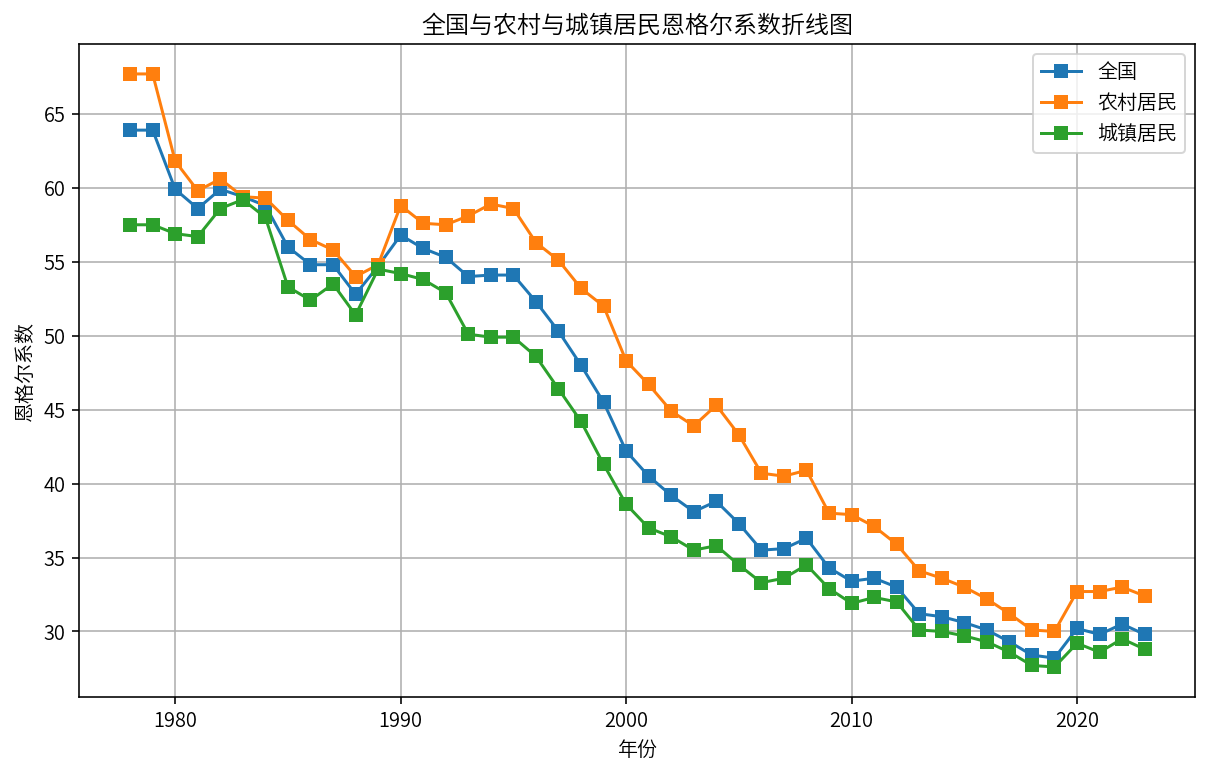
\includegraphics[width=0.65\linewidth]{figures/29.png}
    \caption{农村人民恩格尔系数折线图}
    \label{fig:Engel_coefficient_village}
\end{figure}

图\ref{fig:Engel_coefficient_village}清楚地揭示了过去数十年间我国居民消费结构的显著变化。全国居民的恩格尔系数呈现下降趋势,反映了随着经济的持续发展和人民生活水平的逐步提高,居民的消费结构正在发生深刻变化。这不仅体现了居民生活质量的整体提升,也反映了消费模式的多元化和层次的提升。

特别值得关注的是,农村居民恩格尔系数的显著下降,凸显了农村居民消费结构的重大转变。农村居民的消费不再局限于基本的食品支出,而是更多地向教育、医疗、娱乐等领域扩展此外,城乡居民恩格尔系数之间的差异也在逐渐减小,这一现象不仅显示了城乡居民生活水平的逐步接近,也反映了我国在推动城乡一体化发展、缩小城乡发展差距方面取得的积极进展。